\documentclass[a4paper,10pt]{beamer}
\usepackage[utf8]{inputenc}
\usepackage{color}
\usepackage{colortbl}
\usepackage{xcolor}
\usepackage{caption}
\usepackage{ragged2e}
\usepackage{hyperref}
\usepackage{marvosym}
\renewcommand{\figurename}{Figura}
\usetheme{Warsaw}

%Enumerar figuras
\setbeamertemplate{caption}[numbered]


\logo{
\includegraphics[scale=0.05]{logoUNAM}}
\begin{document}

\begin{frame}
\Large
\title{Tubos fotomultiplicadores y fotodiodos}
\author{Favio Vázquez}
\date{$1^{ro}$ de septiembre de 2015}

Láminas disponibles en \href{https://github.com/FavioVazquez/DeteccionRayosCosmicos-PCF}{(\color{blue} GitHub})

\maketitle
\end{frame}

\section[\'Indice]{}
\frame{

\Large{\'Indice}

\tableofcontents

}

\section{Introducción}
\begin{frame}[allowframebreaks]{Introducción}
\begin{justify}
 El uso masivo de la cuenta de centelladores en la detección y espectroscopia sería 
 imposible sin la disponibilidad de dispositivos que nos permitiera convertir la 
 salida de luz débil de un pulso de centellador, en una señal eléctrica medible. 
 
 \vspace{.3cm}
 
 Los tubos fotomultiplicadores (FM) cumplen con esta tarea muy bien, convirtiendo señales 
 de luz que constan típicamente de no más que unos cientos de fotones, en un pulso 
 de corriente utilizable sin añadir una gran cantidad de ruido aleatorio a la señal.
 
\framebreak

 Existe una gran variedad comercial de estos tubos sensibles a diversas longitudes de onda,
 ultravioleta, luz visible, cercana a la infrarroja y otras del espectro electromagnético.
 
 \vspace{.3cm}
 
 \textbf{Usos}:
 
 \begin{center}
   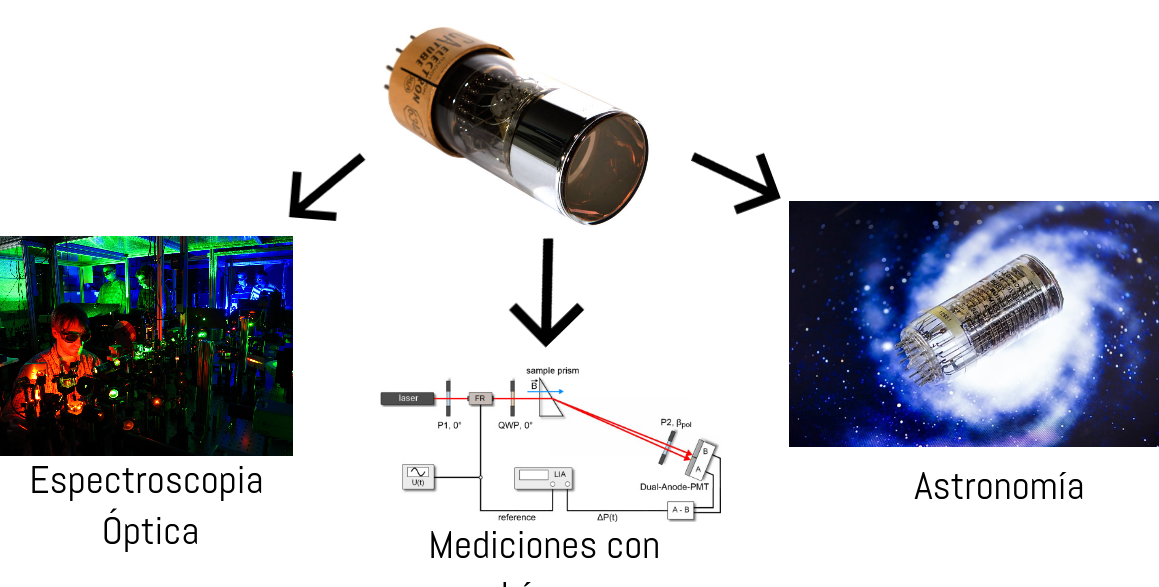
\includegraphics[scale=0.2]{fig1}
 \end{center}

 
 \end{justify}
\end{frame}

\section{Estructura simplificada de un Tubo FM}
\begin{frame}[allowframebreaks]{Estructura simplificada de un Tubo FM}
 
 \begin{columns}[c]
  \column{1.5in}
  \begin{figure}
  \center
   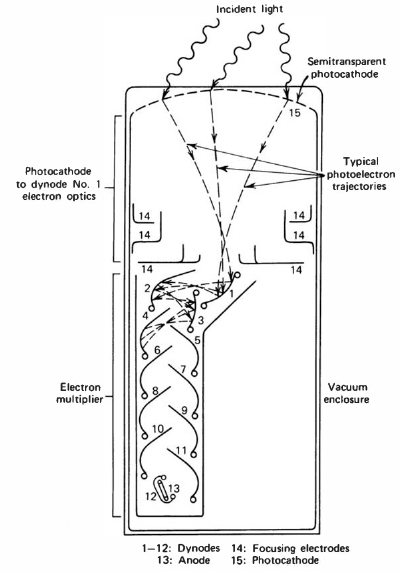
\includegraphics[scale=0.28]{fig2}
   \caption{Elementos básicos de un tubo FM}
  \end{figure}

  \column{2.5in}
  \begin{justify}
   
   \footnotesize{Una envoltura (usualmente de vidrio) sirve como una barrera de presión
   para mantener las condiciones de vacío dentro del tubo, que son requeridas
   para que los electrones de bajas energías puedan ser acelerados eficientemente
   por los campos eléctricos internos.
   
   \vspace{.3cm}
   
   Los dos mayores componentes dentro del tubo son una capa fotosensible, llamada
   el \emph{fotocátodo}, acoplado a una \emph{estructura multiplicadora de fotones}.
   El fotocátodo sirve para convertir la mayor cantidad posible de fotones de luz
   en electrones de baja energía.
   
   \vspace{.3cm}
   
   La sección de multiplicadora de electrones en un tubo FM provee una geometría
   de colección eficiente para los fotoelectrones, y sirve como un amplificador
   casi ideal para incrementar en altas cantidades su número.}
   
   
  \end{justify}

 \end{columns} 
 
 \framebreak
 
  \begin{figure}
  \center
   
\includegraphics[scale=0.4]{fig3}
   \caption{Elementos básicos de un tubo FM}
  \end{figure}
  
  \begin{justify}
   \footnotesize{
   Luego de una amplificación a través de la estructura multiplicadora, un pulso 
   típico de centellador dará lugar a unos $10^7-10^10$ electrones, suficientes
   para servir de señal de carga para el evento original de centelleo. Esta carga
   es colectada convencionalmente en el ánodo o la etapa de salida de la estructura
   multiplicadora.
   
   \vspace{.3cm}
   
   Tubos típicos, cuando son iluminados por un pulso de luz de muy corta duración,
   producirán un pulso de electrones en un tiempo aproximado de unos pocos nanosegundos
   luego de un tiempo de espera de $20-50$ ns.}
   \end{justify}
    
\end{frame}



\end{document}
